%iffalse
\let\negmedspace\undefined
\let\negthickspace\undefined
\documentclass[journal,12pt,onecolumn]{IEEEtran}
\usepackage{cite}
\usepackage{amsmath,amssymb,amsfonts,amsthm}
\usepackage{algorithmic}
\usepackage{graphicx}
\usepackage{textcomp}
\usepackage{xcolor}
\usepackage{txfonts}
\usepackage{listings}
\usepackage{enumitem}
\usepackage{mathtools}
\usepackage{gensymb}
\usepackage{comment}
\usepackage[breaklinks=true]{hyperref}
\usepackage{tkz-euclide} 
\usepackage{listings}
\usepackage{gvv}
\def\inputGnumericTable{}                                 
\usepackage[latin1]{inputenc}                              
\usepackage{color}                                         
\usepackage{array}                                        
\usepackage{longtable}                                     
\usepackage{calc}                                          
\usepackage{multirow}                                      
\usepackage{hhline}                                        
\usepackage{ifthen}                                        
\usepackage{lscape}
\newtheorem{theorem}{Theorem}[section]
\newtheorem{problem}{Problem}
\newtheorem{proposition}{Proposition}[section]
\newtheorem{lemma}{Lemma}[section]
\newtheorem{corollary}[theorem]{Corollary}
\newtheorem{example}{Example}[section]
\newtheorem{definition}[problem]{Definition}
\newcommand{\BEQA}{\begin{eqnarray}}
\newcommand{\EEQA}{\end{eqnarray}}
\newcommand{\define}{\stackrel{\triangle}{=}}
\theoremstyle{remark}
\newtheorem{rem}{Remark}
\graphicspath{ {./Figures/} }
\usepackage{float} % For the [H] float option
\usepackage{textcomp}
\usepackage{multicol}




\begin{document}

\begin{enumerate}[start=1, label=Q.\arabic*]

% Question 1
\item This book, including all its chapters, \underline{\hspace{2cm}} interesting. The students as well as the instructor \underline{\hspace{2cm}} in agreement about it.
    \begin{enumerate}
        \begin{multicols}{2}
        \item is, was
        \item are, are
        \item is, are
        \item were, was
        \end{multicols}
    \end{enumerate}

\hfill{\brak{\text{GATE EE 2020}}}

% Question 2
\item People were prohibited \underline{\hspace{2cm}} their vehicles near the entrance of the main administrative building.
    \begin{enumerate}
        \begin{multicols}{2}
        \item to park
        \item from parking
        \item parking
        \item to have parked
        \end{multicols}
    \end{enumerate}

\hfill{\brak{\text{GATE EE 2020}}}

% Question 3
\item Select the word that fits the analogy:
Do : Undo :: Trust : \underline{\hspace{2cm}}
    \begin{enumerate}
        \begin{multicols}{4}
        \item Entrust
        \item Intrust
        \item Distrust
        \item Untrust
        \end{multicols}
    \end{enumerate}

\hfill{\brak{\text{GATE EE 2020}}}

% Question 4
\item Stock markets \underline{\hspace{2cm}} at the news of the coup.
    \begin{enumerate}
        \begin{multicols}{4}
        \item poised
        \item plunged
        \item plugged
        \item probed
        \end{multicols}
    \end{enumerate}

\hfill{\brak{\text{GATE GA 2020}}}

% Question 5
\item If P, Q, R, S are four individuals, how many teams of size exceeding one can be formed, with Q as a member?
    \begin{enumerate}
        \begin{multicols}{4}
        \item $5$
        \item $6$
        \item $7$
        \item $8$
        \end{multicols}
    \end{enumerate}

\hfill{\brak{\text{GATE GA 2020}}}

% Question 6
\item Non-performing Assets \brak{\text{NPAs}} of a bank in India is defined as an asset, which remains unpaid by a borrower for a certain period of time in terms of interest, principal, or both. Reserve Bank of India \brak{\text{RBI}} has changed the definition of NPA thrice during $1993-2004$, in terms of the holding period of loans. The holding period was reduced by one quarter each time. In $1993$, the holding period was four quarters \brak{360 \text{ days}}.
\par Based on the above paragraph, the holding period of loans in $2004$ after the third revision was \underline{\hspace{2cm}} days.
    \begin{enumerate}
        \begin{multicols}{4}
        \item $45$
        \item $90$
        \item $135$
        \item $180$
        \end{multicols}
    \end{enumerate}

\hfill{\brak{\text{GATE GA 2020}}}

% Question 7
\item Select the next element of the series: Z, WV, RQP, \underline{\hspace{2cm}}
    \begin{enumerate}
        \begin{multicols}{4}
        \item LKJI
        \item JIHG
        \item KJIH
        \item NMLK
        \end{multicols}
    \end{enumerate}

\hfill{\brak{\text{GATE GA 2020}}}

% Question 8
\item In four-digit integer numbers from $1001$ to $9999$, the digit group "$37$" \brak{\text{in the same sequence}} appears \underline{\hspace{2cm}} times.
    \begin{enumerate}
        \begin{multicols}{4}
        \item $270$
        \item $279$
        \item $280$
        \item $299$
        \end{multicols}
    \end{enumerate}

\hfill{\brak{\text{GATE GA 2020}}}

% Question 9
\item Given a semicircle with O as the centre, as shown in the figure, the ratio $\frac{\overline{AC}+\overline{CB}}{\overline{AB}}$ is \underline{\hspace{2cm}} where $\overline{AC}$, $\overline{CB}$ and $\overline{AB}$ are chords.
\begin{figure}[H]
    \centering
    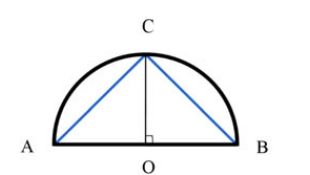
\includegraphics[width=0.4\columnwidth]{Figures/aq9.png}
    \caption{}
\end{figure}
    \begin{enumerate}
        \begin{multicols}{4}
        \item $\sqrt{2}$
        \item $\sqrt{3}$
        \item $2$
        \item $3$
        \end{multicols}
    \end{enumerate}

\hfill{\brak{\text{GATE GA 2020}}}

% Question 10
\item The revenue and expenditure of four different companies P, Q, R and S in $2015$ are shown in the figure. If the revenue of company Q in $2015$ was $20\%$ more than that in $2014$, and company Q had earned a profit of $10\%$ on expenditure in $2014$, then its expenditure \brak{\text{in million rupees}} in $2014$ was \underline{\hspace{2cm}}.
\begin{figure}[H]
    \centering
    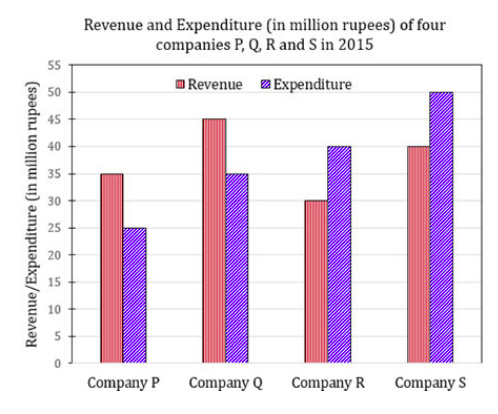
\includegraphics[width=0.6\columnwidth]{Figures/aq10.png}
    \caption{}
\end{figure}
    \begin{enumerate}
        \begin{multicols}{2}
        \item $32.7$
        \item $33.7$
        \item $34.1$
        \item $35.1$
        \end{multicols}
    \end{enumerate}

\hfill{\brak{\text{GATE GA 2020}}}

% Question 11
\item $ax^{3}+bx^{2}+cx+d$ is a polynomial on real $x$ over real coefficients $a, b, c, d$ wherein $a \ne 0$. Which of the following statements is true?
    \begin{enumerate}
        \item d can be chosen to ensure that $x=0$ is a root for any given set a, b, c.
        \item No choice of coefficients can make all roots identical.
        \item a, b, c, d can be chosen to ensure that all roots are complex.
        \item c alone cannot ensure that all roots are real.
    \end{enumerate}

\hfill{\brak{\text{GATE EE 2020}}}

% Question 12
\item Which of the following is true for all possible non-zero choices of integers $m, n; m \ne n$, or all possible non-zero choices of real numbers $p, q; p \ne q$, as applicable?
    \begin{enumerate}
        \item $\frac{1}{\pi}\int_{0}^{\pi}\sin m\theta \sin n\theta d\theta=0$
        \item $\frac{1}{2\pi}\int_{-\pi/2}^{\pi/2}\sin p\theta \sin q\theta d\theta=0$
        \item $\frac{1}{2\pi}\int_{-\pi}^{\pi}\sin p\theta \cos q\theta d\theta=0$
        \item $\lim_{\alpha\rightarrow\infty}\frac{1}{2\alpha}\int_{-\alpha}^{\alpha}\sin p\theta \sin q\theta d\theta=0$
    \end{enumerate}

\hfill{\brak{\text{GATE EE 2020}}}

% Question 13
\item Which of the following statements is true about the two sided Laplace transform?
    \begin{enumerate}
        \item It exists for every signal that may or may not have a Fourier transform.
        \item It has no poles for any bounded signal that is non-zero only inside a finite time interval.
        \item The number of finite poles and finite zeroes must be equal.
        \item If a signal can be expressed as a weighted sum of shifted one sided exponentials, then its Laplace Transform will have no poles.
    \end{enumerate}

\hfill{\brak{\text{GATE EE 2020}}}

% Question 14
\item Consider a signal $x[n]=\brak{\frac{1}{2}}^{n}1[n],$ where $1[n]=0$ if $n<0$ and $1[n]=1$ if $n \ge 0$. The z-transform of $x[n-k],$ $k>0$ is $\frac{z^{-k}}{1-\frac{1}{2}z^{-1}}$ with region of convergence being \underline{\hspace{2cm}}.
    \begin{enumerate}
        \begin{multicols}{2}
        \item $\abs{z}<2$
        \item $\abs{z}>2$
        \item $\abs{z}<1/2$
        \item $\abs{z}>1/2$
        \end{multicols}
    \end{enumerate}

\hfill{\brak{\text{GATE EE 2020}}}

% Question 15
\item The value of the following complex integral, with C representing the unit circle centered at origin in the counterclockwise sense, is:
\begin{align*}
\int_{c}\frac{z^{2}+1}{z^{2}-2z}dz
\end{align*}
    \begin{enumerate}
        \begin{multicols}{2}
        \item $8\pi i$
        \item $-8\pi i$
        \item $-\pi i$
        \item $\pi i$
        \end{multicols}
    \end{enumerate}

\hfill{\brak{\text{GATE EE 2020}}}

% Question 16
\item $\chi_{R}$ and $x_{A}$ are, respectively, the rms and average values of $x\brak{t}=x\brak{t-T}$, and similarly, $y_{R}$ and $y_{A}$ are, respectively, the rms and average values of $y\brak{t}=kx\brak{t}$. k, T are independent of t. Which of the following is true?
    \begin{enumerate}
        \begin{multicols}{2}
        \item $y_{A}=kx_{A}; y_{R}=kx_{R}$
        \item $y_{A}=kx_{A}; y_{R}\ne kx_{R}$
        \item $y_{A}\ne kx_{A}; y_{R}=kx_{R}$
        \item $y_{A}\ne kx_{A}; y_{R}\ne kx_{R}$
        \end{multicols}
    \end{enumerate}

\hfill{\brak{\text{GATE EE 2020}}}

% Question 17
\item A three-phase cylindrical rotor synchronous generator has a synchronous reactance $X_{s}$ and a negligible armature resistance. The magnitude of per phase terminal voltage is $V_{A}$ and the magnitude of per phase induced emf is $E_{A}$. Considering the following two statements, P and Q,
\par P: For any three-phase balanced leading load connected across the terminals of this synchronous generator, $V_{A}$ is always more than $E_{A}$.
\par Q: For any three-phase balanced lagging load connected across the terminals of this synchronous generator, $V_{A}$ is always less than $E_{A}$.
\par which of the following options is correct?
    \begin{enumerate}
        \item P is false and Q is true.
        \item P is true and Q is false.
        \item P is false and Q is false.
        \item P is true and Q is true.
    \end{enumerate}

\hfill{\brak{\text{GATE EE 2020}}}

% Question 18
\item A lossless transmission line with $0.2$ pu reactance per phase uniformly distributed along the length of the line, connecting a generator bus to a load bus, is protected up to $80\%$ of its length by a distance relay placed at the generator bus. The generator terminal voltage is $1$ pu. There is no generation at the load bus. The threshold pu current for operation of the distance relay for a solid three phase-to-ground fault on the transmission line is closest to:
    \begin{enumerate}
        \begin{multicols}{2}
        \item $1.00$
        \item $3.61$
        \item $5.00$
        \item $6.25$
        \end{multicols}
    \end{enumerate}

\hfill{\brak{\text{GATE EE 2020}}}

% Question 19
\item Out of the following options, the most relevant information needed to specify the real power \brak{P} at the PV buses in a load flow analysis is
    \begin{enumerate}
        \item solution of economic load dispatch
        \item rated power output of the generator
        \item rated voltage of the generator
        \item base power of the generator
    \end{enumerate}

\hfill{\brak{\text{GATE EE 2020}}}

% Question 20
\item Consider a linear time-invariant system whose input $r\brak{t}$ and output $y\brak{t}$ are related by the following differential equation:
\begin{align*}
\frac{d^{2}y\brak{t}}{dt^{2}}+4y\brak{t}=6r\brak{t}
\end{align*}
The poles of this system are at
    \begin{enumerate}
        \begin{multicols}{2}
        \item $+2j, -2j$
        \item $+2, -2$
        \item $+4, -4$
        \item $+4j, -4j$
        \end{multicols}
    \end{enumerate}

\hfill{\brak{\text{GATE EE 2020}}}

% Question 21
\item A single-phase, full-bridge diode rectifier fed from a $230$ V, $50$ Hz sinusoidal source supplies a series combination of finite resistance, R, and a very large inductance, L. The two most dominant frequency components in the source current are:
    \begin{enumerate}
        \begin{multicols}{2}
        \item $50$ Hz, $0$ Hz
        \item $50$ Hz, $100$ Hz
        \item $50$ Hz, $150$ Hz
        \item $150$ Hz, $250$ Hz
        \end{multicols}
    \end{enumerate}

\hfill{\brak{\text{GATE EE 2020}}}

% Question 22
\item Thyristor $T_{1}$ is triggered at an angle $\alpha$ \brak{\text{in degree}}, and $T_{2}$ at angle $180\degree+\alpha$, in each cycle of the sinusoidal input voltage. Assume both thyristors to be ideal. To control the load power over the range $0$ to $2$ kW, the minimum range of variation in $\alpha$ is:
\begin{figure}[H]
    \centering
    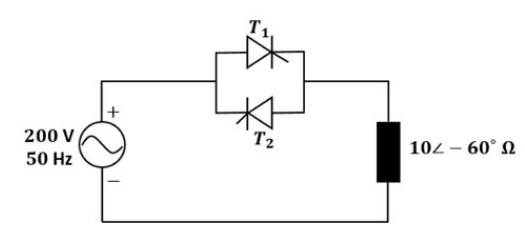
\includegraphics[width=0.5\columnwidth]{Figures/aq12.png}
    \caption{}
\end{figure}
    \begin{enumerate}
        \begin{multicols}{2}
        \item $0\degree$ to $60\degree$
        \item $0\degree$ to $120\degree$
        \item $60\degree$ to $120\degree$
        \item $60\degree$ to $180\degree$
        \end{multicols}
    \end{enumerate}

\hfill{\brak{\text{GATE EE 2020}}}

% Question 23
\item Which of the options is an equivalent representation of the signal flow graph shown here?
\begin{figure}[H]
    \centering
    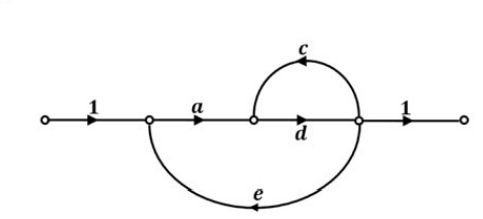
\includegraphics[width=0.6\columnwidth]{Figures/aq13.png}
    \caption{}
\end{figure}
    \begin{enumerate}
    
        \item 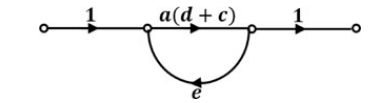
\includegraphics[width=0.8\columnwidth]{Figures/aq13A.png}
        \item 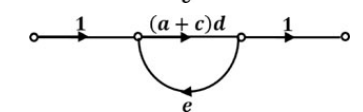
\includegraphics[width=0.8\columnwidth]{Figures/aq13B.png}
        \item 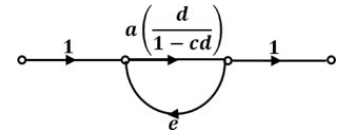
\includegraphics[width=0.8\columnwidth]{Figures/aq13C.png}
        \item 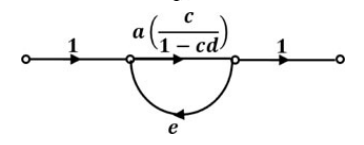
\includegraphics[width=0.8\columnwidth]{Figures/aq13D.png}
        
    \end{enumerate}

\hfill{\brak{\text{GATE EE 2020}}}

% Question 24
\item A common-source amplifier with a drain resistance, $R_{D}=4.7 \text{ k}\ohm$, is powered using a $10$ V power supply. Assuming that the transconductance, $g_{m}$, is $520 \mu\text{A/V}$, the voltage gain of the amplifier is closest to:
    \begin{enumerate}
        \begin{multicols}{2}
        \item $-2.44$
        \item $-1.22$
        \item $1.22$
        \item $2.44$
        \end{multicols}
    \end{enumerate}

\hfill{\brak{\text{GATE EE 2020}}}

% Question 25
\item A sequence detector is designed to detect precisely $3$ digital inputs, with overlapping sequences detectable. For the sequence ($1,0,1$) and input data ($1,1,0,1,0,0,1,1,0,1,0,1,1,0$), what is the output of this detector?
    \begin{enumerate}
        \begin{multicols}{2}
        \item $1,1,0,0,0,0,1,1,0,1,0,0$
        \item $0,1,0,0,0,0,0,1,0,1,0,0$
        \item $0,1,0,0,0,0,0,1,0,1,1,0$
        \item $0,1,0,0,0,0,0,0,1,0,0,0$
        \end{multicols}
    \end{enumerate}

\hfill{\brak{\text{GATE EE 2020}}}

\item Consider the initial value problem below. The value of y at $x = \ln 2$, \brak{rounded off to 3 decimal places} is \underline{\hspace{2cm}}.
\begin{align*}
\frac{dy}{dx} = 2x - y, \quad y\brak{0} = 1
\end{align*}

\hfill{\brak{\text{GATE EE 2020}}}

% Question 57
\item A three-phase, $50$ Hz, $4$-pole induction motor runs at no-load with a slip of $1$ \%. With full load, the slip increases to $5$ \%. The \% speed regulation of the motor \brak{rounded off to 2 decimal places} is \underline{\hspace{2cm}}.

\hfill{\brak{\text{GATE EE 2020}}}

% Question 58
\item Currents through ammeters A2 and A3 in the figure are $1\angle10\degree$ and $1\angle70\degree$, respectively. The reading of the ammeter A1rounded off to 3 decimal places is \underline{\hspace{2cm}} A.
\begin{figure}[H]
    \centering
    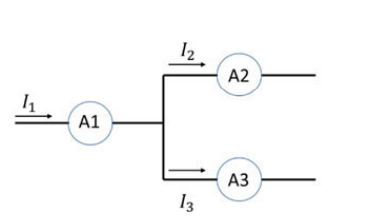
\includegraphics[width=0.4\columnwidth]{Figures/b28.png}
    \caption{}
\end{figure}

\hfill{\brak{\text{GATE EE 2020}}}

\item The Thevenin equivalent voltage, $V_{TH}$, in V \brak{rounded off to 2 decimal places} of the network shown below, is \underline{\hspace{2cm}}.
\begin{figure}[H]
    \centering
    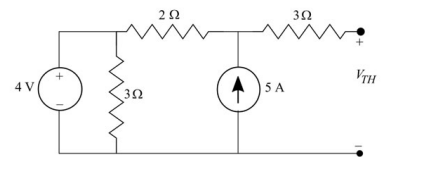
\includegraphics[width=0.6\columnwidth]{Figures/299.png}
    \caption{}
\end{figure}

\hfill{\brak{\text{GATE EE 2020}}}

\item A double pulse measurement for an inductively loaded circuit controlled by the IGBT switch is carried out to evaluate the reverse recovery characteristics of the diode, D, represented approximately as a piecewise linear plot of current vs time at diode turn-off. $L_{par}$ is a parasitic inductance due to the wiring of the circuit, and is in series with the diode. The point on the plot \brak{indicate your choice by entering 1, 2, 3 or 4} at which the IGBT experiences the highest current stress is \underline{\hspace{2cm}}.
\begin{figure}[H]
    \centering
    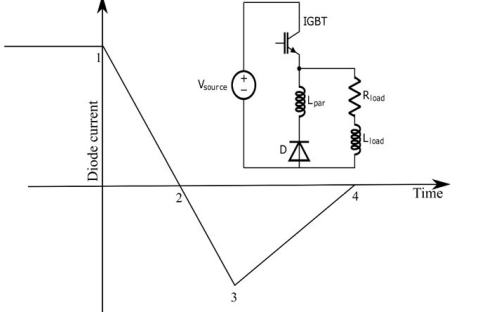
\includegraphics[width=0.8\columnwidth]{Figures/30.png}
    \caption{}
\end{figure}

\hfill{\brak{\text{GATE EE 2020}}}

% Question 61
\item A single-phase, 4 kVA, 200 V/100 V, 50 Hz transformer with laminated CRGO steel core has rated no-load loss of 450 W. When the high-voltage winding is excited with 160 V, 40 Hz sinusoidal ac supply, the no-load losses are found to be 320 W. When the high-voltage winding of the same transformer is supplied from a 100 V, 25 Hz sinusoidal ac source, the no-load losses will be \underline{\hspace{2cm}} W \brak{rounded off to 2 decimal places}.

\hfill{\brak{\text{GATE EE 2020}}}

\item A single-phase inverter is fed from a 100 V dc source and is controlled using a quasi-square wave modulation scheme to produce an output waveform, $v(t)$, as shown. The angle $\sigma$ is adjusted to entirely eliminate the $3^{rd}$ harmonic component from the output voltage. Under this condition, for $v(t)$, the magnitude of the $5^{th}$ harmonic component as a percentage of the magnitude of the fundamental component is \underline{\hspace{2cm}} \brak{rounded off to 2 decimal places}.
\begin{figure}[H]
    \centering
    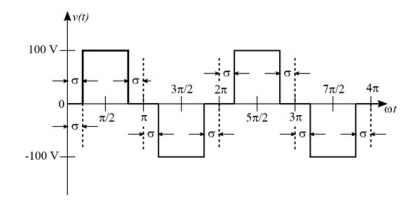
\includegraphics[width=0.7\columnwidth]{Figures/b32.png}
    \caption{}
\end{figure}

\hfill{\brak{\text{GATE EE 2020}}}

% Question 63
\item A single 50 Hz synchronous generator on droop control was delivering 100 MW power to a system. Due to increase in load, generator power had to be increased by 10 MW, as a result of which, system frequency dropped to 49.75 Hz. Further increase in load in the system resulted in a frequency of 49.25 Hz. At this condition, the power in MW supplied by the generator is \underline{\hspace{2cm}} \brak{rounded off to 2 decimal places}.

\hfill{\brak{\text{GATE EE 2020}}}

% Question 64
\item Consider a negative unity feedback system with forward path transfer function 
\[
G\brak{s} = \frac{K}{\brak{s+a}\brak{s-b}\brak{s+c}},
\] 
where $K, a, b, c$ are positive real numbers. For a Nyquist path enclosing the entire imaginary axis and right half of the $s$-plane in the clockwise direction, the Nyquist plot of $\brak{1+G\brak{s}}$, encircles the origin of $\brak{1+G\brak{s}}$-plane once in the clockwise direction and never passes through this origin for a certain value of $K$. Then, the number of poles of $\dfrac{G\brak{s}}{1+G\brak{s}}$ lying in the open right half of the $s$-plane is \underline{\hspace{2cm}}.
\hfill \brak{\text{GATE EE 2020}}

\item The cross-section of a metal-oxide-semiconductor structure is shown schematically. Starting from an uncharged condition, a bias of $+3$ V is applied to the gate contact with respect to the body contact. The charge inside the silicon dioxide layer is then measured to be $+Q$. The total charge contained within the dashed box shown, upon application of bias, expressed as a multiple of $Q$ \brak{absolute value in Coulombs, rounded off to the nearest integer} is \underline{\hspace{2cm}}.
\begin{figure}[H]
    \centering
    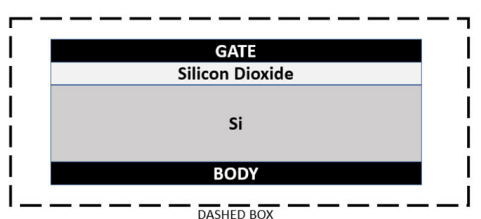
\includegraphics[width=0.6\columnwidth]{Figures/35.png}
    \caption{}
\end{figure}

\hfill{\brak{\text{GATE EE 2020}}}

\item For real numbers, $x$ and $y$, with $y=3x^{2}+3x+1$, the maximum and minimum value of $y$ for $x \in [-2,0]$ are respectively.
    \begin{enumerate}
        \begin{multicols}{2}
        \item $7$ and $1/4$
        \item $7$ and $1$
        \item $-2$ and $-1/2$
        \item $1$ and $1/4$
        \end{multicols}
    \end{enumerate}

    \hfill{\brak{\text{GATE EE 2020}}}

    \item The vector function expressed by $F=a_{x}\brak{5y-k_{1}z}+a_{y}\brak{3z+k_{2}x}+a_{z}\brak{k_{3}y-4x}$ represents a conservative field, where $a_{x}, a_{y}, a_{z}$ are unit vectors along x, y and z directions, respectively. The values of constants $k_{1}, k_{2}, k_{3}$ are given by:
    \begin{enumerate}
        \begin{multicols}{2}
        \item $k_{1}=3, k_{2}=3, k_{3}=7$
        \item $k_{1}=3, k_{2}=8, k_{3}=5$
        \item $k_{1}=4, k_{2}=5, k_{3}=3$
        \item $k_{1}=0, k_{2}=0, k_{3}=0$
        \end{multicols}
    \end{enumerate}

    \hfill{\brak{\text{GATE EE 2020}}}

    \item A $250$ V dc shunt motor has an armature resistance of $0.2~\ohm$ and a field resistance of $100~\ohm$. When the motor is operated on no-load at rated voltage, it draws an armature current of $5$ A and runs at $1200$ rpm. When a load is coupled to the motor, it draws total line current of $50$ A at rated voltage, with a $5\%$ reduction in the air-gap flux due to armature reaction. Voltage drop across the brushes can be taken as $1$ V per brush under all operating conditions. The speed of the motor, in rpm, under this loaded condition, is closest to:
    \begin{enumerate}
        \begin{multicols}{4}
        \item $1200$
        \item $1000$
        \item $1220$
        \item $900$
        \end{multicols}
    \end{enumerate}

    \hfill{\brak{\text{GATE EE 2020}}}
\item Two buses, i and j, are connected with a transmission line of admittance Y, at the two ends of which there are ideal transformers with turns ratios as shown. Bus admittance matrix for the system is:
    \begin{figure}[H]
        \centering
        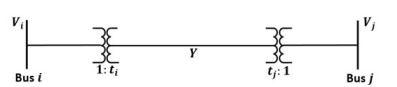
\includegraphics[width=0.6\columnwidth]{Figures/39.png}
        \caption{}
    \end{figure}
    \begin{enumerate}
        \item $\myvec{-t_{i}t_{j}Y & t_{j}^{2}Y \\ t_{i}^{2}Y & -t_{i}t_{j}Y}$
        \item $\myvec{t_{i}t_{j}Y & -t_{j}^{2}Y \\ -t_{i}^{2}Y & t_{i}t_{j}Y}$
        \item $\myvec{t_{i}^{2}Y & -t_{i}t_{j}Y \\ -t_{i}t_{j}Y & t_{j}^{2}Y}$
        \item $\myvec{-t_{i}^{2}Y & t_{i}t_{j}Y \\ t_{i}t_{j}Y & -t_{j}^{2}Y}$
    \end{enumerate}

    \hfill{\brak{\text{GATE EE 2020}}}

    \item Consider the diode circuit shown below. The diode, D, obeys the current-voltage characteristic $I_D = I_S \brak{\exp\brak{\frac{V_D}{nV_T}} - 1}$, where $n>1$, $V_T>0$, $V_D$ is the voltage across the diode and $I_D$ is the current through it. The circuit is biased so that voltage, $V>0$ and current, $I<0$. If you had to design this circuit to transfer maximum power from the current source $I_1$ to a resistive load \brak{\text{not shown}} at the output, what values of $R_1$ and $R_2$ would you choose\brak{\text{?}}

\begin{enumerate}
\begin{multicols}{2}
\item Large $R_1$ and large $R_2$.
\item Small $R_1$ and small $R_2$.
\item Large $R_1$ and small $R_2$.
\item Small $R_1$ and large $R_2$.
\end{multicols}
\end{enumerate}

\begin{figure}[H]
\centering
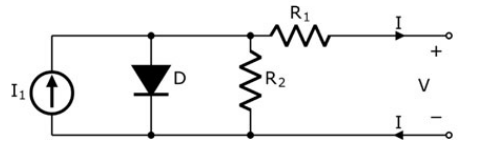
\includegraphics[width=0.6\columnwidth]{qs40.png}
\caption{}
\end{figure}
\hfill \brak{\text{GATE EE 2020}}


%Question X+1
\item A non-ideal diode is biased with a voltage of $-0.03 \, V$, and a diode current of $I_1$ is measured. The thermal voltage is $26 \, mV$ and the ideality factor for the diode is $15/13$. The voltage, in V, at which the measured current increases to $1.5 I_1$, is closest to
\begin{enumerate}
\begin{multicols}{2}
\item $-0.02$
\item $-0.09$
\item $-1.50$
\item $-4.50$
\end{multicols}
\end{enumerate}
\hfill \brak{\text{GATE EE 2020}}


%Question X+2
\item A benchtop dc power supply acts as an ideal $4 \, A$ current source as long as its terminal voltage is below $10 \, V$. Beyond this point, it begins to behave as an ideal $10 \, V$ voltage source for all load currents going down to $0 \, A$. When connected to an ideal rheostat, find the load resistance value at which maximum power is transferred, and the corresponding load voltage and current.
\begin{enumerate}
\item Short, $0 \, \ohm, 10 \, V$
\item Open, $4 \, A, 0 \, V$
\item $2.5 \, \ohm, 4 \, A, 10 \, V$
\item $2.5 \, \ohm, 4 \, A, 5 \, V$
\end{enumerate}
\hfill \brak{\text{GATE EE 2020}}


%Question X+3
\item The static electric field inside a dielectric medium with relative permittivity, $\epsilon_r = 2.25$, expressed in cylindrical coordinate system is given by the following expression
\[
\mathbf{E} = a_r \, 2r + a_\varphi \, \brak{\frac{3}{r}} + a_z \, 6
\]
where $a_r, a_\varphi, a_z$ are unit vectors along $r, \varphi$ and $z$ directions, respectively. If the above expression represents a valid electrostatic field inside the medium, then the volume charge density associated with this field in terms of free space permittivity, $\epsilon_0$, in SI units is given by\brak{\text{:}}
\begin{enumerate}
\item 3$\epsilon$
\item 4$\epsilon$
\item 5$\epsilon$
\item 9$\epsilon$
\end{enumerate}
\hfill \brak{\text{GATE EE 2020}}

%Question 34
\item Consider a permanent magnet dc \brak{\text{PMDC}} motor which is initially at rest. At $t=0$, a dc voltage of $5 \, V$ is applied to the motor. Its speed monotonically increases from $0 \, \text{rad/s}$ to $6.32 \, \text{rad/s}$ in $0.5 \, s$ and finally settles to $10 \, \text{rad/s}$. Assuming that the armature inductance of the motor is negligible, the transfer function for the motor is
\begin{enumerate}
\begin{multicols}{2}
\item $\dfrac{10}{0.5s+1}$
\item $\dfrac{2}{0.5s+1}$
\item $\dfrac{2}{s+0.5}$
\item $\dfrac{10}{s+0.5}$
\end{multicols}
\end{enumerate}
\hfill \brak{\text{GATE EE 2020}}


%Question 35
\item Which of the following options is correct for the system shown below?

\begin{figure}[H]
\centering
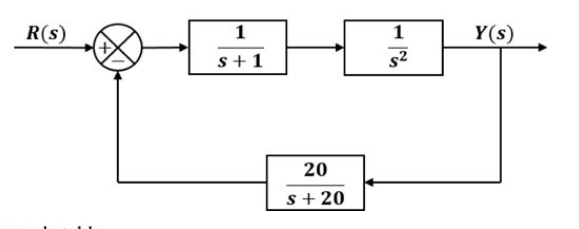
\includegraphics[width=0.7\columnwidth]{qs45.png}
\caption{}
\end{figure}

\begin{enumerate}
\begin{multicols}{2}
\item 4th order and stable
\item 3rd order and stable
\item 4th order and unstable
\item 3rd order and unstable
\end{multicols}
\end{enumerate}
\hfill \brak{\text{GATE EE 2020}}


%Question 36
\item Consider a negative unity feedback system with the forward path transfer function
\[
\dfrac{s^2+ s + 1}{s^3+2s^2+2s+K},
\]
where $K$ is a positive real number. The value of $K$ for which the system will have some of its poles on the imaginary axis is \underline{\hspace{2cm}}.
\begin{enumerate}
\begin{multicols}{2}
\item 9
\item 8
\item 7
\item 6
\end{multicols}
\end{enumerate}
\hfill \brak{\text{GATE EE 2020}}


%Question 37
\item Suppose for input $x(t)$ a linear time-invariant system with impulse response $h(t)$ produces output $y(t)$, so that $x(t) * h(t) = y(t)$. Further, if $\abs{x(t)} * \abs{h(t)} = z(t)$, which of the following statements is true?
\begin{enumerate}
\item For all $t \in \brak{-\infty, \infty}, z(t) \leq y(t)$
\item For some but not all $t \in \brak{-\infty, \infty}, z(t) \leq y(t)$
\item For all $t \in \brak{-\infty, \infty}, z(t) \geq y(t)$
\item For some but not all $t \in \brak{-\infty, \infty}, z(t) \geq y(t)$
\end{enumerate}
\hfill \brak{\text{GATE EE 2020}}


%Question 38
\item The causal realization of a system transfer function $H(s)$ having poles at $\brak{2,-1}, \brak{-2,1}$ and zeroes at $\brak{2,1}, \brak{-2,-1}$ will be
\begin{enumerate}
\begin{multicols}{2}
\item stable, real, allpass
\item unstable, complex, allpass
\item unstable, real, highpass
\item stable, complex, lowpass
\end{multicols}
\end{enumerate}
\hfill \brak{\text{GATE EE 2020}}

\item Which of the following options is true for a linear time-invariant discrete time system that obeys the difference equation
\[
y[n] - a y[n-1] = b_0 x[n] - b_1 x[n-1]
\]
$y[n]$ is unaffected by the values of $x[n-k]; k>2$. \\
The system is necessarily causal. \\
The system impulse response is non-zero at infinitely many instants. \\
When $x[n]=0, n<0$, the function $y[n]; n>0$ is solely determined by the function $x[n]$.
\begin{enumerate}
\begin{multicols}{4}
\item Only 1
\item Only 2
\item Only 3
\item Only 4
\end{multicols}
\end{enumerate}
\hfill \brak{\text{GATE EE 2020}}


%Question X+1
\item Let $a_r, a_\varphi$ and $a_z$ be unit vectors along $r, \varphi$ and $z$ directions, respectively in the cylindrical coordinate system. For the electric flux density given by 
\[
\mathbf{D} = \brak{a_r \, 15 + a_\varphi \, 2r - a_z \, 3r z} \, \text{Coulomb/m}^2,
\] 
the total electric flux, in Coulomb, emanating from the volume enclosed by a solid cylinder of radius $3\, m$ and height $5\, m$ oriented along the $z$-axis with its base at the origin is\brak{:}
\begin{enumerate}
\begin{multicols}{2}
\item $54\pi$
\item $90\pi$
\item $108\pi$
\item $180\pi$
\end{multicols}
\end{enumerate}
\hfill \brak{\text{GATE EE 2020}}


%Question X+2
\item A stable real linear time-invariant system with single pole at $p$, has a transfer function 
\[
H(s) = \frac{s^2+100}{s-p}
\]
with a dc gain of $5$. The smallest positive frequency, in rad/s, at unity gain is closest to\brak{:}
\begin{enumerate}
\begin{multicols}{2}
\item $8.84$
\item $11.08$
\item $78.13$
\item $122.87$
\end{multicols}
\end{enumerate}
\hfill \brak{\text{GATE EE 2020}}


%Question X+3
\item The number of purely real elements in a lower triangular representation of the given $3\times3$ matrix, obtained through the given decomposition is \underline{\hspace{2cm}}.
\[
\myvec{2 & 3 & 2 \\ 3 & 2 & 1 \\ 3 & 1 & 7} 
= 
\myvec{a_{11} & 0 & 0 \\ a_{12} & a_{22} & 0 \\ a_{13} & a_{23} & a_{33}}
\myvec{a_{11} & a_{12} & a_{13} \\ 0 & a_{22} & a_{23} \\ 0 & 0 & a_{33}}^T
\]
\begin{enumerate}
\begin{multicols}{4}
\item 5
\item 6
\item 8
\item 9
\end{multicols}
\end{enumerate}
\hfill \brak{\text{GATE EE 2020}}

\item The figure below shows the per-phase Open Circuit Characteristics (measured in V) and Short Circuit Characteristics (measured in A) of a $14$ kVA, $400$ V, $50$ Hz, $4$-pole, $3$-phase, delta connected alternator, driven at $1500$ rpm. The field current, $I_f$ is measured in A. Readings taken are marked as respective (x, y) coordinates in the figure. Ratio of the unsaturated and saturated synchronous impedances $(Z_s(\text{unsat}) / Z_s(\text{sat}))$ the alternator is closest to:
    \begin{figure}[H]
        \centering
        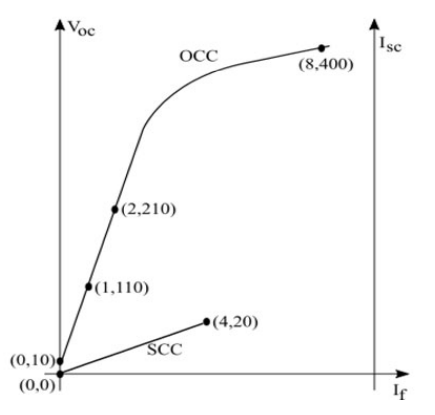
\includegraphics[width=0.6\columnwidth]{Figures/qs53.png}
        \caption{}
    \end{figure}
    \begin{enumerate}
        \item $2.100$
        \item $2.025$
        \item $2.000$
        \item $1.000$
    \end{enumerate}

    \hfill{\brak{\text{GATE EE 2020}}}

    \item Let $\hat{a}_x$ and $\hat{a}_y$ be unit vectors along x and y directions, respectively. A vector function is given by
    \[ \vec{F} = \hat{a}_y y - \hat{a}_x x \]
    The line integral of the above function
    \[ \int_C \vec{F} \cdot d\vec{l} \]
    along the curve C, which follows the parabola $y=x^2$ as shown below is \underline{\hspace{2cm}} \brak{rounded off to 2 decimal places}.
    \begin{figure}[H]
        \centering
        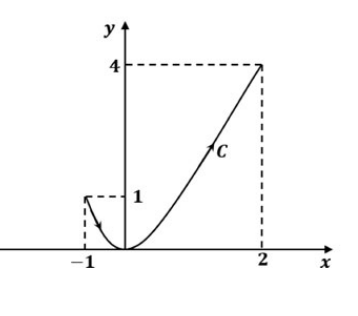
\includegraphics[width=0.4\columnwidth]{Figures/qs54.png}
        \caption{}
    \end{figure}

    \hfill{\brak{\text{GATE EE 2020}}}

    \item A resistor and a capacitor are connected in series to a $10$ V dc supply through a switch. The switch is closed at $t=0$, and the capacitor voltage is found to cross $0$ V at $t=0.4\tau$, where $\tau$ is the circuit time constant. The absolute value of percentage change required in the initial capacitor voltage if the zero crossing has to happen at $t=0.2\tau$ is \underline{\hspace{2cm}} \brak{rounded off to 2 decimal places}.

    \hfill{\brak{\text{GATE EE 2020}}}

    \item The figure below shows the per-phase Open Circuit Characteristics (measured in V) and Short Circuit Characteristics (measured in A) of a $14$ kVA, $400$ V, $50$ Hz, $4$-pole, $3$-phase, delta connected alternator, driven at $1500$ rpm. The field current, $I_f$ is measured in A. Readings taken are marked as respective (x, y) coordinates in the figure. Ratio of the unsaturated and saturated synchronous impedances $(Z_s(\text{unsat}) / Z_s(\text{sat}))$ of the alternator is closest to:
    \begin{figure}[H]
        \centering
        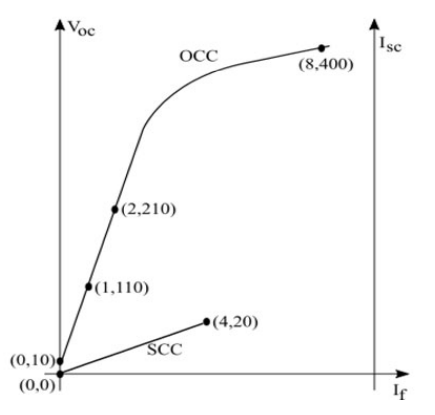
\includegraphics[width=0.6\columnwidth]{Figures/qs53.png}
        \caption{}
    \end{figure}
    \begin{enumerate}
        \item $2.100$
        \item $2.025$
        \item $2.000$
        \item $1.000$
    \end{enumerate}

    \hfill{\brak{\text{GATE EE 2020}}}

    \item Let $\hat{a}_x$ and $\hat{a}_y$ be unit vectors along x and y directions, respectively. A vector function is given by
    \[ \vec{F} = \hat{a}_y y - \hat{a}_x x \]
    The line integral of the above function
    \[ \int_C \vec{F} \cdot d\vec{l} \]
    along the curve C, which follows the parabola $y=x^2$ as shown below is \underline{\hspace{2cm}} \brak{rounded off to 2 decimal places}.
    \begin{figure}[H]
        \centering
        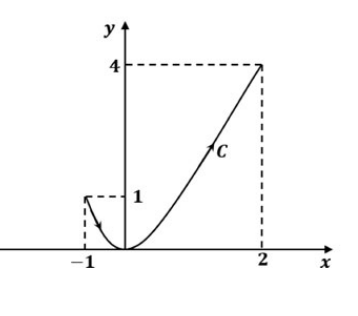
\includegraphics[width=0.4\columnwidth]{Figures/qs54.png}
        \caption{}
    \end{figure}

    \hfill{\brak{\text{GATE EE 2020}}}

    \item A resistor and a capacitor are connected in series to a $10$ V dc supply through a switch. The switch is closed at $t=0$, and the capacitor voltage is found to cross $0$ V at $t=0.4\tau$, where $\tau$ is the circuit time constant. The absolute value of percentage change required in the initial capacitor voltage if the zero crossing has to happen at $t=0.2\tau$ is \underline{\hspace{2cm}} \brak{rounded off to 2 decimal places}.

    \hfill{\brak{\text{GATE EE 2020}}}

    \item A cylindrical rotor synchronous generator with constant real power output and constant terminal voltage is supplying $100$ A current to a $0.9$ lagging power factor load. An ideal reactor is now connected in parallel with the load, as a result of which the total lagging reactive power requirement of the load is twice the previous value while the real power remains unchanged. The armature current is now \underline{\hspace{2cm}} A \brak{rounded off to 2 decimal places}.

    \hfill{\brak{\text{GATE EE 2020}}}

    \item Bus 1 with voltage magnitude $V_1 = 1.1$ pu is sending reactive power $Q_{12}$ towards bus 2 with voltage magnitude $V_2 = 1$ pu through a lossless transmission line of reactance X. Keeping the voltage at bus 2 fixed at 1 pu, magnitude of voltage at bus 1 is changed, so that the reactive power $Q_{12}$ sent from bus 1 is increased by $20\%$. Real power flow through the line under both the conditions is zero. The new value of the voltage magnitude, $V_1$, in pu \brak{rounded off to 2 decimal places}, at bus 1 is \underline{\hspace{2cm}}.
    \begin{figure}[H]
        \centering
        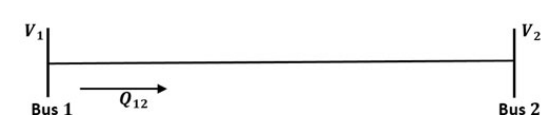
\includegraphics[width=0.5\columnwidth]{Figures/qs60.png}
        \caption{}
    \end{figure}

    \hfill{\brak{\text{GATE EE 2020}}}

    \item Windings A, B and C have $20$ turns each and are wound on the same iron core as shown, along with winding X which has $2$ turns. The figure shows the sense (clockwise/anti-clockwise) of each of the windings only and does not reflect the exact number of turns. If windings A, B and C are supplied with balanced 3-phase voltages at $50$ Hz and there is no core saturation, the no-load RMS voltage (in V, rounded off to 2 decimal places) across winding X is \underline{\hspace{2cm}}.
    \begin{figure}[H]
        \centering
        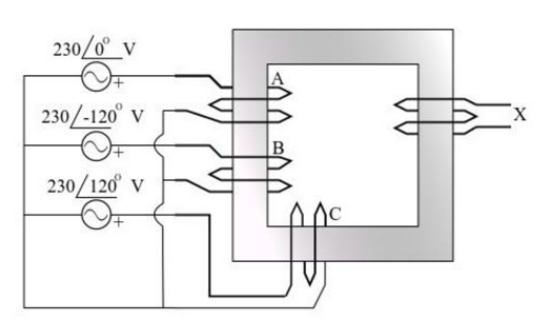
\includegraphics[width=0.6\columnwidth]{Figures/qs61.png}
        \caption{}
    \end{figure}

    \hfill{\brak{\text{GATE EE 2020}}}

    \item A cylindrical rotor synchronous generator has steady state synchronous reactance of $0.7$ pu and subtransient reactance of $0.2$ pu. It is operating at ($1+j0$) pu terminal voltage with an internal emf of ($1+j0.7$) pu. Following a three-phase solid short circuit fault at the terminals of the generator, the magnitude of the subtransient internal emf (rounded off to 2 decimal places) is \underline{\hspace{2cm}} pu.

    \hfill{\brak{\text{GATE EE 2020}}}

    \item In the dc-dc converter circuit shown, switch Q is switched at a frequency of $10$ kHz with a duty ratio of $0.6$. All components of the circuit are ideal, and the initial current in the inductor is zero. Energy stored in the inductor in mJ \brak{rounded off to 2 decimal places} at the end of $10$ complete switching cycles is \underline{\hspace{2cm}}.
    \begin{figure}[H]
        \centering
        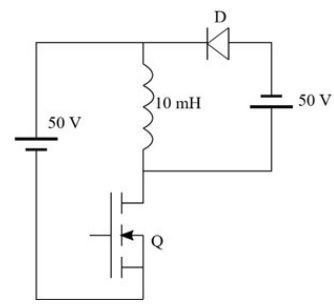
\includegraphics[width=0.4\columnwidth]{Figures/qs63.png}
        \caption{}
    \end{figure}

    \hfill{\brak{\text{GATE EE 2020}}}

    \item A single-phase, full-bridge, fully controlled thyristor rectifier feeds a load comprising a $10~\ohm$ resistance in series with a very large inductance. The rectifier is fed from an ideal $230$ V, $50$ Hz sinusoidal source through cables which have negligible internal impedance and a total inductance of $2.28$ mH. If the thyristors are triggered at an angle $\alpha = 45\degree$, the commutation overlap angle in degree \brak{rounded off to 2 decimal places} is \underline{\hspace{2cm}}.

    \hfill{\brak{\text{GATE EE 2020}}}

    \item A non-ideal Si-based pn junction diode is tested by sweeping the bias applied across its terminals from $-5$ V to $+5$ V. The effective thermal voltage, $V_T$, for the diode is measured to be ($29 \pm 2$) mV. The resolution of the voltage source in the measurement range is $1$ mV. The percentage uncertainty (rounded off to 2 decimal places) in the measured current at a bias voltage of $0.02$ V is \underline{\hspace{2cm}}.

    \hfill{\brak{\text{GATE EE 2020}}}


\item The temperature of the coolant oil bath for a transformer is monitored using the circuit shown. It contains a thermistor with a temperature-dependent resistance, $R_{\text{thermistor}} = 2(1+\alpha T)$ k$\ohm$, where T is the temperature in $\degree$C. The temperature coefficient, $\alpha$, is $-(4 \pm 0.25)$ $\%/\degree$C. Circuit parameters: $R_1 = 1$ k$\ohm$, $R_2 = 1.3$ k$\ohm$, $R_3 = 2.6$ k$\ohm$. The error in the output signal (in V, rounded off to 2 decimal places) at $150\degree$C is \underline{\hspace{2cm}}.
    \begin{figure}[H]
        \centering
        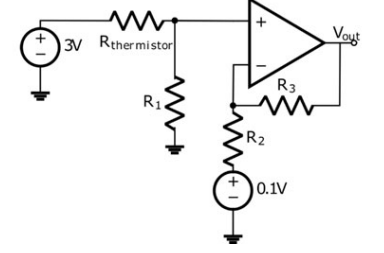
\includegraphics[width=0.6\columnwidth]{Figures/qs66.png}
        \caption{}
    \end{figure}

    \hfill{\brak{\text{GATE EE 2020}}}
     \item An $8085$ microprocessor accesses two memory locations ($2001\text{H}$) and ($2002\text{H}$), that contain $8$-bit numbers $98\text{H}$ and B$1\text{H}$, respectively. The following program is executed:
    
    \begin{verbatim}
LXI H,2001H
MVI A, 21H
INX H
ADD M
INX H
MOV M, A
HLT
    \end{verbatim}
    
    At the end of this program, the memory location $2003\text{H}$ contains the number in decimal \brak{\text{base }10} form \underline{\hspace{2cm}}.
    
    \hfill{\brak{\text{GATE EE 2020}}}

    \item A conducting square loop of side length $1$ m is placed at a distance of $1$ m from a long straight wire carrying a current $I = 2$ A as shown below. The mutual inductance, in nH \text(rounded off to  2 decimal places), between the conducting loop and the long wire is \underline{\hspace{2cm}}.
    
    \begin{figure}[H]
        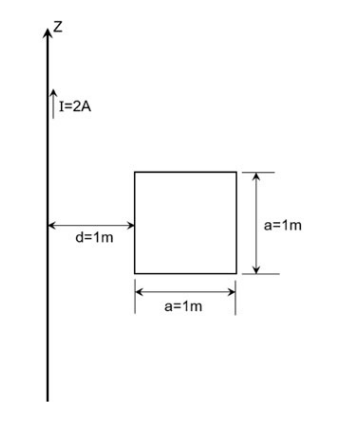
\includegraphics[width=0.4\columnwidth]{Figures/qs68.png}
        \centering
        \caption{}
    \end{figure}
    
    \hfill{\brak{\text{GATE EE 2020}}}

\end{enumerate}
\end{document}
